\documentclass[12pt, a4paper]{article}
\usepackage[utf8]{inputenc}
% \usepackage[russian]{babel}
\usepackage[pdftex]{graphicx, color}
\usepackage{amsmath, amsfonts, amssymb, amsthm}
\usepackage{bm}
\usepackage[left=2cm,right=2cm,top=1.5cm,bottom=2cm]{geometry}
\usepackage{indentfirst}
\usepackage{hyperref}
\usepackage{float}
\usepackage[table,xcdraw]{xcolor}
\usepackage{tikz}
\usepackage[justification=centering,labelfont=bf]{caption}
\usepackage{multirow}
\usetikzlibrary{quotes,arrows.meta}

\graphicspath{{pics/}}

\begin{document}
    \begin{center}
        
\includegraphics[height=3cm]{UVM}

        {\large\textbf{
            CS352 Evolutionary Computation: Homework 2
        }}

        \vspace{0.3cm}

        \textit{\textbf{Ayat Ospanov}}

        \today
    \end{center}

    \tableofcontents

    \section{Task 1}
        The equation for the basic Schema Theorem is the next:
        \begin{align*}
            E[m(H, t+1)] \geq m(H, t) \frac{f(H)}{\bar{f}} \Big(1 - \frac{\delta(H)}{L - 1}p_c - o(H) p_m\Big)
        \end{align*}
        where
        \begin{itemize}
            \item $m(H, t)$ is the proportion of individuals representing schema H at time-step $t$
            \item $f(H)$ is the fitness of the schema H
            \item $\bar{f}$ is the mean fitness of the population
            \item $o(H)$ is the order of the schema H
            \item $\delta(H)$ is the defining length of the schema H
            \item $L$ is the length of a genotype
            \item $p_c$ is the probability of applying crossover
            \item $p_m$ is the bitwise mutation probability
        \end{itemize}

        The first factor $m(H, t) \frac{f(H)}{\bar{f}}$ is the probability of a
        schema being selected. It is obvious that it depends on the relative fitness
        of the schema (because the selection is fitness proportionate) and on the
        proportion of individuals.

        The second factor $1 - \frac{\delta(H)}{L - 1} p_c - o(H) p_m$ is the
        probability of surviving variation operators. $\frac{\delta(H)}{L - 1} p_c$
        is the probability of disrupting examples by crossover and $o(H) p_m$ is the
        probability of disrupting examples by mutation.

        Thus, the theorem states ``short, low-order (derives from the second factor)
        schemata with above-average fitness (the first factor) increase exponentially
        over generations''

    \section{Task 2}
        The fundamental message of the Schema Theorem, or Building Block Hypothesis,
        is that GAs can begin by selecting short, low-order schemata examples, and
        then combine them to create higher order schemata, repeating until a schema
        of length $L-1$ and order $L$ is created and selected.

    \section{Task 3}
        There are 3 types of problem ``difficulty''.
        \begin{itemize}
            \item intra-BB
            \item inter-BB
            \item extra-BB
        \end{itemize}
        The most important is an intra-BB difficulty, or deceptiveness. This means
        at least one optimal schema is outcompeted by non-optimal schema.

    \section{Task 4}
        \begin{align*}
            S1 &= \texttt{*0**11***0**}, & o(S1) = 4, \delta(S1) = 8, L = 12\\
            S2 &= \texttt{*****0*1****}, & o(S1) = 2, \delta(S1) = 2, L = 12
        \end{align*}

        {\bf a)} The probability $p_s$ of surviving both crossover and mutation is
        $$p_s(H) = (1 - p_m)^{o(H)}\Big(1 - p_c \frac{\delta(H)}{L - 1}\Big)$$

        Thus,
        \begin{align*}
            p_s(S1) &= (1 - p_m)^4 (1 - \frac{8 p_c}{11})\\
            p_s(S2) &= (1 - p_m)^2 (1 - \frac{2 p_c}{11})
        \end{align*}

        It is obvious, that $p_s(S1) \leq p_s(S2)$. And the probability of
        surviving of both of them is $p_s(S1) \cdot p_s(S2)$

        {\bf b)} As we know, ``building blocks'' are short (in terms of defining
        length) and low-order schematas. $S1$ cannot be called a ``building
        block'' as its order and length are high, while $S2$ can be called
        a ``building block'', because it has the length of 2 and the order
        of 2 which makes possible to describe $S2$ as short and low-order
        schemata.

    \section{Task 5}
        \begin{table}[H]
        \centering
            \begin{tabular}{ll}
            \rowcolor[HTML]{C0C0C0}
            string & fitness \\
            100    & 10      \\
            111    & 20      \\
            011    & 15      \\
            010    & 15
            \end{tabular}
        \end{table}

        {\bf a)}
        \begin{align*}
            f(1**) &= \frac{N_{100} f_{100} + N_{111} f(111)}{N_{100} + N_{111}} =\\
            &= \frac{25 * 10 + 25 * 20}{25 + 25} = \frac{10 + 20}{2} = 15
        \end{align*}

        {\bf b)}
        The estimated number of samples of a schemata H at the next step is:
        $$n(H, t+1) = n(H, t) \frac{f(H)}{\bar{f}}$$
        Thus, for the schemata \texttt{1**} we can get the estimated number of samples
        on the next step:
        $$n(\texttt{1**}, t+1) = 50 * \frac{15}{15} = 50$$

        But we need the estimated fitness. To count, we need to estimate the number
        of survivors of guys from the schema \texttt{1**}. As we know those guys and can
        estimate numbers for a scheme, we can put $H_1 = 100$ and $H_2 = 111$. Now
        let's estimate the numbers:
        \begin{align*}
            n(100, t+1) &= n(100, t) \frac{f(100)}{\bar{f}} = 25 \cdot \frac{10}{15} = 25 \cdot \frac{2}{3}\\
            n(111, t+1) &= n(111, t) \frac{f(111)}{\bar{f}} = 25 \cdot \frac{20}{15} = 25 \cdot \frac{4}{3}
        \end{align*}

        Now we can estimate the fitness value for the \texttt{1**} scheme.
        \begin{align*}
            f_{t+1}(\texttt{1**}) &= \frac{n(100, t+1) * f(100) + n(111, t+1) * f(111)}{n(100, t+1) + n(111, t+1)} =\\
            &= \frac{25 \cdot \frac{2}{3} \cdot 10 + 25 \cdot \frac{4}{3} \cdot 20}{50}
            = \frac{\frac{2}{3} \cdot 10 + \frac{4}{3} \cdot 20}{2} =\\
            &= \frac{10 + 2 \cdot 20}{3} = \frac{100}{6} \approx 16.7\\
        \end{align*}

    \section{Task 6}
        \begin{table}[H]
        \centering
            \begin{tabular}{l|l|llllllll}
            \multicolumn{2}{l|}{phenotype (integer)} & 0   & 1   & 2   & 3   & 4   & 5   & 6   & 7   \\ \hline
            \multirow{2}{*}{genotype}    & binary    & 000 & 001 & 010 & 011 & 100 & 101 & 110 & 111 \\
                                         & gray      & 000 & 001 & 011 & 010 & 110 & 111 & 101 & 100 \\ \hline
            \multicolumn{2}{l|}{fitness}             & 7   & 5   & 3   & 9   & 10  & 1   & 6   & 6
            \end{tabular}
        \end{table}

        \begin{table}[H]
        \centering
        \caption{Schema Analysis for binary code and gray code}
        \label{tab:sa}
            \begin{tabular}{|l|l|c|ccc|ccc|c|}
            \hline
                                    & order   & 3          & \multicolumn{3}{c|}{2}                 & \multicolumn{3}{c|}{1}                 & 0              \\ \hline
            \multicolumn{10}{|c|}{} \\ \hline
            \multirow{8}{*}{binary} & schema  & 111        & 11*        & 1*1        & *11          & **1          & *1*        & 1**        & ***            \\
                                    & fitness & \textbf{6} & \textbf{6} & 3.5        & 7.5          & 5.25         & \textbf{6} & 5.75       & \textbf{5.875} \\ \cline{2-10}
                                    & schema  &            & 01*        & 0*1        & *01          & **0          & *0*        & 0**        &                \\
                                    & fitness &            & \textbf{6} & 7          & 3            & \textbf{6.5} & 5.75       & \textbf{6} &                \\ \cline{2-10}
                                    & schema  &            & 10*        & 1*0        & *10          &              &            &            &                \\
                                    & fitness &            & 5.5        & \textbf{8} & 4.5          &              &            &            &                \\ \cline{2-10}
                                    & schema  &            & 00*        & 0*0        & *00          &              &            &            &                \\
                                    & fitness &            & \textbf{6} & 5          & \textbf{8.5} &              &            &            &                \\ \hline
            \multicolumn{10}{|c|}{} \\ \hline
            \multirow{8}{*}{gray}   & schema  & 100        & 10*        & 1*0        & *00          & 1**          & *0*        & **0        & ***            \\
                                    & fitness & \textbf{6} & \textbf{6} & \textbf{8} & \textbf{6.5} & 5.75         & \textbf{6} & \textbf{8} & \textbf{5.875} \\ \cline{2-10}
                                    & schema  &            & 11*        & 1*1        & *11          & 0**          & *1*        & **1        &                \\
                                    & fitness &            & 5.5        & 3.5        & 2            & \textbf{6}   & 5.75       & 3.75       &                \\ \cline{2-10}
                                    & schema  &            & 01*        & 0*1        & *01          &              &            &            &                \\
                                    & fitness &            & \textbf{6} & 4          & 5.5          &              &            &            &                \\ \cline{2-10}
                                    & schema  &            & 00*        & 0*0        & *00          &              &            &            &                \\
                                    & fitness &            & \textbf{6} & \textbf{8} & \textbf{6.5} &              &            &            &                \\ \hline
            \end{tabular}
        \end{table}

        \begin{figure}[H]
            \centering
            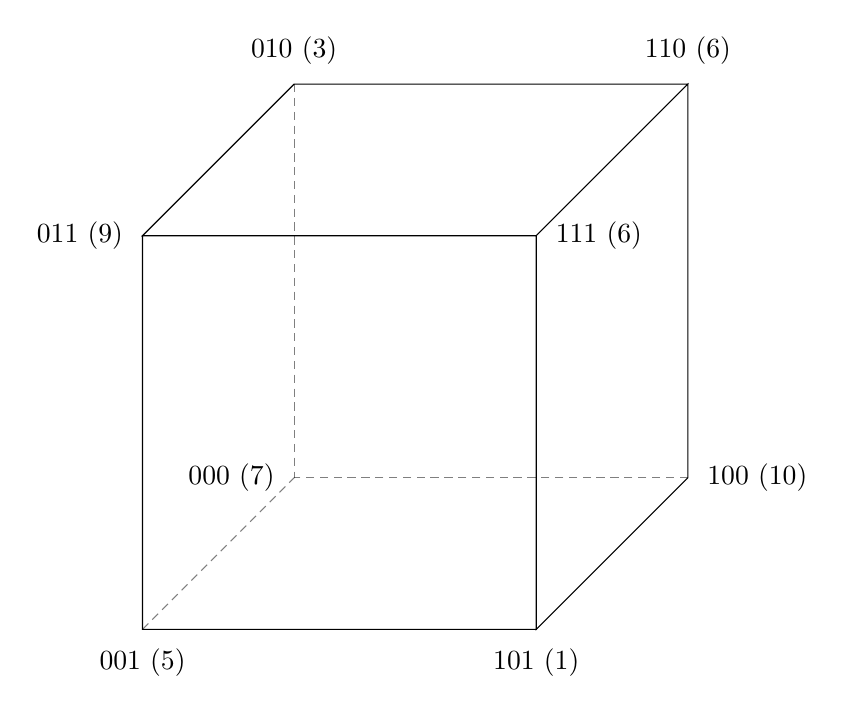
\begin{tikzpicture}[every edge quotes/.append style={auto, text=blue}]
                \pgfmathsetmacro{\cubex}{5}
                \pgfmathsetmacro{\cubey}{5}
                \pgfmathsetmacro{\cubez}{5}
                \draw [draw=black, every edge/.append style={draw=black, densely dashed, opacity=.5}]
                    (0,0,0) coordinate (o) -- ++(-\cubex,0,0) coordinate (a) -- ++(0,-\cubey,0) coordinate (b) edge coordinate [pos=1] (g) ++(0,0,-\cubez)  -- ++(\cubex,0,0) coordinate (c) -- cycle
                    (o) -- ++(0,0,-\cubez) coordinate (d) -- ++(0,-\cubey,0) coordinate (e) edge (g) -- (c) -- cycle
                    (o) -- (a) -- ++(0,0,-\cubez) coordinate (f) edge (g) -- (d) -- cycle;
                \node[label=right:111 (6)] at (o) {};
                \node[label=left:011 (9)] at (a) {};
                \node[label=below:001 (5)] at (b) {};
                \node[label=below:101 (1)] at (c) {};
                \node[label=above:110 (6)] at (d) {};
                \node[label=right:100 (10)] at (e) {};
                \node[label=above:010 (3)] at (f) {};
                \node[label=left:000 (7)] at (g) {};
            \end{tikzpicture}
            \caption{Hamming cube diagram for binary encoding}
            \label{fig:hamm_bin}
        \end{figure}

        \begin{figure}[H]
            \centering
            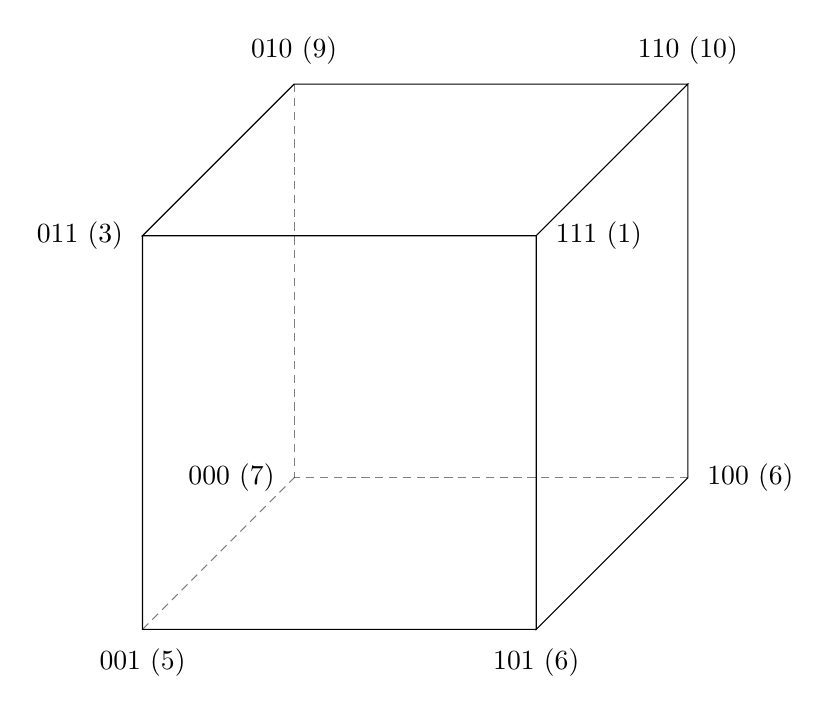
\begin{tikzpicture}[every edge quotes/.append style={auto, text=blue}]
                \pgfmathsetmacro{\cubex}{5}
                \pgfmathsetmacro{\cubey}{5}
                \pgfmathsetmacro{\cubez}{5}
                \draw [draw=black, every edge/.append style={draw=black, densely dashed, opacity=.5}]
                    (0,0,0) coordinate (o) -- ++(-\cubex,0,0) coordinate (a) -- ++(0,-\cubey,0) coordinate (b) edge coordinate [pos=1] (g) ++(0,0,-\cubez)  -- ++(\cubex,0,0) coordinate (c) -- cycle
                    (o) -- ++(0,0,-\cubez) coordinate (d) -- ++(0,-\cubey,0) coordinate (e) edge (g) -- (c) -- cycle
                    (o) -- (a) -- ++(0,0,-\cubez) coordinate (f) edge (g) -- (d) -- cycle;
                \node[label=right:111 (1)] at (o) {};
                \node[label=left:011 (3)] at (a) {};
                \node[label=below:001 (5)] at (b) {};
                \node[label=below:101 (6)] at (c) {};
                \node[label=above:110 (10)] at (d) {};
                \node[label=right:100 (6)] at (e) {};
                \node[label=above:010 (9)] at (f) {};
                \node[label=left:000 (7)] at (g) {};
            \end{tikzpicture}
            \caption{Hamming cube diagram for gray encoding}
            \label{fig:hamm_gray}
        \end{figure}
\end{document}
